%  Typ dokumentu - článek, prezentace aj.
\documentclass[english]{article}

%  Nastaví vstupní a výstupní kódování znaků (encoding) a lokalizace
\usepackage[T1]{fontenc}
\usepackage[utf8]{inputenc}
\usepackage[english,czech]{babel}
\usepackage{icomma}

%  Formát papíru a odsazení od jeho okrajů
\usepackage[letterpaper]{geometry}
\geometry{verbose,tmargin=1.5cm,bmargin=2cm,lmargin=2cm,rmargin=2cm}

%  Umožňuje pracovat s grafikou
\usepackage{graphicx}
\usepackage{bigstrut}
\usepackage{epstopdf}

%  Automaticky odsadí i první paragraf v každé sekci
\usepackage{indentfirst}

%  Umožňuje rozdělovat obsah na více sloupců
\usepackage{multicol}
\usepackage{booktabs}
\usepackage{pgffor}

%  Umožňuje používat hypertextové odkazy, nastavuje jejich barvu a vlastnosti
\usepackage[unicode]{hyperref}
\hypersetup{
	colorlinks=true, citecolor=blue, filecolor=blue, linkcolor=blue,
	urlcolor=blue
}

%  Umožnění odstranění italiky u jednotek
\newcommand{\unit}[1]{~\mathrm{#1}}
\newcommand{\unitb}[1]{~\mathrm{[#1]}}
\newcommand{\unitbr}[1]{\qquad\mathrm{[#1]}}

%  Formátování stránek, empty = odstraní číslování
% \pagestyle{empty}

%  Řádkování
\linespread{1.2}

%  Lepší zobrazování matematiky (rozšíření sum o \limits atd.)
%  Umožní psát přes \mathbb{N/R/Q/..} množiny čísel
\everymath{\displaystyle}
\usepackage{amsmath, amsthm, amssymb, wasysym}

%  Velikost fontu matematických výrazů v dokumentu lze pro danou
% základního fontu dokumentu upravit pomocí:
% \DeclareMathSizes{X}{Y}{Z}{U} kde:
% X je velikost fontu v dokumentu, pro kterou se matematika upraví
% Y je standartní velikost fontu matematiky
% Z je velikost fontu zmenšených (vnořených výrazů)
% U je velikost fontu ještě více zmenšených (vnořených výrazů).
\DeclareMathSizes{10}{10.5}{9}{9}

%  Nastaví autora, název, datum, skupinu měření apod. 
%  (můj vlastní příkaz, umožní znovu-použití v dokumentu)
\newcommand{\Author}{David Roesel}
\newcommand{\Coauthor}{Schönfeldová} %, Vyšín}
\newcommand{\Institute}{FJFI ČVUT v Praze}
\newcommand{\Subject}{VAKUOVÁ FYZIKA A TECHNIKA}
\newcommand{\Group}{Pá 14:30}
\newcommand{\Kruh}{FE}
\newcommand{\Title}{Úloha \#5  \\Turbomolekulární vývěva, analýza zbyt. plynů}
\newcommand{\Date}{5.12.2014}

% Custom comands
\newcommand{\dd}{\mathrm{d}}
\newcommand{\dln}{\mathrm{ln}}
\newcommand{\ee}{\mathrm{e}}
\newcommand{\degc}{^\circ C}
\newcommand{\jelina}{Oooo, Jelina!}

% Začátek dokumentu - Formátování na výstup
\begin{document}

% Interní proměnné, možno zobrazovat u prezentací, používají se při
% generování pomocí \titlepage apod.
\author{\Author}
\title{\Title}
\date{\Date}

%  Lokalizace některých názvů do češtiny
\renewcommand{\figurename}{Obr.}
\renewcommand{\tablename}{Tab.}
\renewcommand{\refname}{Reference}

% --- Hlavička dokumentu -----------------------------------------------

\setlength{\parindent}{0cm}
\begin{multicols}{2}
\textbf{\Subject \\
        \Institute \\[0.1cm]
%\large  \Title \\[0.5cm]
\Title \\[0.5cm]
}
\begin{tabular}{rlrl}
\large Datum měření: & \Date & \large Skupina: & \Group \\
\large Jméno: & \Author & \large Kroužek:  & \Kruh\\
\large Spolupracovali: & \Coauthor &\large Klasifikace:\\
\end{tabular}

\begin{flushright}

\includegraphics[scale=0.28]{../../_meta/fjfi_standart.pdf}
\hspace{0.2cm}

\includegraphics[scale=0.28]{../../_meta/cvut_standart.pdf}
\end{flushright}
\end{multicols}
\hrule
\vspace{0.5cm}

% ----------------------------------------------------------------------


% --- Tělo dokumentu ---------------------------------------------------
\setlength{\parindent}{0.5cm}

\section{Pracovní úkoly}

\begin{enumerate}
	\item Sledujte čerpání uzavřeného objemu membránovou a turbomolekulární vývěvou. \\Zaznamenejte závislost $p = \mathrm{f(}t\mathrm{)}$.
	\item Zaznamenejte hmotnostní spektrum zbytkového plynu a určete hlavní převládající plyny ve zbytkové atmosféře.
	\item Sledujte časový vývoj tlaku vybraných plynů.
	\item Zapněte vyhřívaní recipientu (do teploty $\leq 100\unit{\degc}$) a sledujte časový průběh tlaku vybraných plynů (až do $100\unit{\degc}$ + cca. 20 min). Vypněte ohřev a pokračujte ve sledování $p\mathrm{(}t\mathrm{)}$.
	\item Ofukujte napouštěcí špunt heliem a sledujte $p\mathrm{(He)} = \mathrm{f(}t\mathrm{)}$.
	\item Sledujte vliv otáček na parciální tlaky plynů zbytkové atmosféry.
\end{enumerate}

\section{Úvod}
	Turbomolekulární vývěva (TMV) je transportní vývěva, v níž molekuly plynu získávají přídavnou složku rychlosti přenosem impulsu od povrchu rychle se pohybujících lopatek rotoru. Následně jsou vedeny systémem statorů a dalších rotorů. Lopatky rotorů a statorů jsou mírně nakloněny v závislosti na pozici ve vývěvě a jsou vždy nakloněny opačným směrem než lopatky předchozí vrstvy. Otáčky pumpy dosahují řádově tisíců až desítek tisíc za vteřinu a jsou drahé na výrobu či opravu. Používají se však v laboratořích velmi často, jelikož čerpají rychle a s menším potřebným příkonem, než například vývěvy difusní. Ač je dosahované vakuum velmi čisté, pro lehké molekuly má TMV nízký kompresní poměr.

\section{Vypracování}
    \subsection{Teoretický úvod}
    		Turbomolekulární vývěvy se vyrábějí jak pro vysoké, tak pro ultravysoké vakuum a jejich čerpací rychlosti se pohybují od desítek do tisíců l/s. Každý litr za sekundu čerpací rychlosti cenově odpovídá zhruba jednomu tisíci Kč. Při normálním provozu mají na výstupu tlak řádově v jednotkách Pa. 
    		
    		Pro správnou funkci TMV je třeba splnit podmínku molekulárního proudění plynu uvnitř, a je tedy zvykem předřazovat TMV rotační či jinou vývěvu, která zajistí příslušný výstupní tlak. Pro dobré fungování vývěvy musí být rychlost lopatek rotoru srovnatelná s rychlostí tepelného pohybu molekul $v_s$ čerpaného vzduchu. To se dá snadněji splnit pro těžší složky vzduchu, hůře to tím pádem jde pro lehké plyny jako je $\mathrm{H_2}$, pro které jsou hodnoty $v_s$ rovny 471 a 1755~m/s \cite{bib:praskripta}. TMV mají typicky otáčky rotoru o velikosti desítek tisíc za minutu, což odpovídá při rotoru o průměru 10~cm obvodové rychlosti okolo 470~m/s. Kompresní poměr TMV závisí podstatně na poměru této rychlosti s rychlostí tepelného pohybu molekul $v_s$, což je vidět například na tom, že pro dusík dosahuje přibližně hodnot řádu $10^{-9}$, zatímco pro vodík pouhých $10^{-4}$. Pro dobré vakuum je tedy třeba TMV předřadit vývěvu, která zajistí pokles parciálního tlaku vodíku. V našem případě se jednalo o vývěvu membránovou.
    		
    		Mimo tento vliv je rychlost čerpání TMV téměř nezávislá na druhu čerpaného plynu a závisí pouze na geometrii lopatek a jejich rychlosti. Maximální čerpací rychlosti se dosahuje v momentu, kdy všechny stupně TMV pracují v podmínkách molekulárního proudění. Konstrukční provedení TMV bývá buď jedno- a nebo dvouproudové, které se liší hlavně v orientaci rotoru. Při vypuštění vývěvy je třeba ji napustit suchým vzduchem, aby nedošlo ke vzlínání oleje po odplyněném povrchu. Někdy je třeba kompenzovat vibrace, které TMV při svém provozu generuje.
    
    \subsection{Postup měření}	
    	\subsubsection{Čerpání pomocí TMV}
	    	Když jsme k úloze přišli, byla aparatura již sestavena. Měření tlaku v recipientu bylo automaticky přepínáno mezi dvěma různými způsoby měření a vakuometr stačilo pouze zapnout. Otevřeli jsme napouštěcí ventil na zadní části TMV a nechali napustit recipient vzduchem. Počkali jsme, než se tlak uvnitř ustálil nebo přelezl rozsah stupnice (vakuometr pak ukazoval \texttt{or}). Poté jsme zavřeli napouštěcí ventil, zapnuli hlavní vypínač TMV a čerpání (jak TMV, tak membránovou vývěvou). Od momentu zapnutí jsme začali sledovat a zaznamenávat průběh tlaku v čerpaném objemu v závislosti na čase. 
	
		\subsubsection{Hmotnostní spektrum zbytkového plynu}
			Poté jsme si pečlivě prostudovali důležité stránky z manuálu k programu $\mathrm{Talk~Star}$ a po dosažení dostatečně nízkého tlaku (menšího než $10^{-3}$) jsme ho zapnuli, čímž se zapnul také kvadrupol v aparatuře. Následně jsme v programu provedli záznam hmotnostního spektra zbytkového plynu (režim ,,Scan``) a výsledná data jsme uložili a převedli do \texttt{ASCII} formátu.
			
		\subsubsection{Časový vývoj parciálních tlaků}
			Následně jsme přepnuli v programu $\mathrm{Talk~Star}$ režim na ,,Trend 2``, jelikož původní režim ,,Trend`` vedl k opakovaným pádům programu, a začali jsme sledovat vývoj tlaku vybraných plynů v čase. Zaznamenali jsme jistý časový interval a výsledná data jsme opět uložili a převedli do \texttt{ASCII} formátu. 
			
			Poté jsme zapnuli vyhřívání recipientu a dále jsme sledovali vývoj parciálních tlaků jednotlivých plynů až do dosažení $100\unit{\degc}$. Poté jsme nechali aparaturu zahřátou po dobu přibližně 20 minut a pak jsme zahřívání vypnuli a čekali na ustálení parciálních tlaků. 
		
		\subsubsection{Ofukování napouštěcího šroubu heliem}
			Za sledování vybraných plynů jsme pootevřeli napouštěcí ventil na zadní straně TMV tak, aby se změna neprojevila na hodnotách v grafu. Následně jsme ofukovali ventil heliem z balonku a sledovali změny na grafu v režimu ,,Trend 2``. Průběh parciálních tlaků jsme zaznamenávali a po ukončení ofukování jsme data opět uložili a převedli.
			
		\subsubsection{Vliv otáček TMV na parciální tlaky}
			Následně jsme se připravili na nový záznam v režimu ,,Trend 2`` a ve stejný moment jsme zahájili měření na počítači a vypnuli čerpání turbomolekulární vývěvou. Vypnutí mělo za následek pokles otáček a my jsme sledovali a zaznamenávali vývoj parciálních tlaků v čase. V momentu, kdy tlak v recipientu stoupl nad $10^{-3}\unit{Pa}$, jsme čerpání opět zapnuli, aby nedošlo k poškození kvadrupolu. Po návratu otáček na původní maximální hodnotu 1500~Hz jsme ukončili záznam a naměřená data uložili a převedli.
			
			Po ukončení tohoto měření jsme zaznamenaná data odeslali na svůj počítač, vypnuli jsme kvadrupol a TMV pomocí obou vypínačů.
		
	\subsection{Naměřené hodnoty}
		\subsubsection{Čerpání pomocí TMV}
			Naměřený průběh logaritmu tlaku v závislosti na čase je vynesen do grafu na Obr.~\ref{fig:g_lnp}.
			
		\subsubsection{Hmotnostní spektrum zbytkového plynu}
			Zaznamenané hmotnostní spektrum zbytkového plynu je vyneseno do grafu na Obr.~\ref{fig:g_spektrum}.
			
		\subsubsection{Časový vývoj parciálních tlaků}
			Záznam z režimu ,,Trend 2`` programu $\mathrm{Talk~Star}$ je vynesen do grafu na Obr.~\ref{fig:g_trend}. Ke všem hodnotám byl přičten dvojnásobek absolutní hodnoty nejnižšího naměřeného záznamu pro helium, jelikož je pro něj kvadrupol špatně zkalibrovaný a záporné hodnoty by se nám při logaritmickém měřítku nezobrazily.
			
			Při vyhřívání aparatury jsme pozorovali mírný nárůst parciálních tlaků. Po zhruba deseti minutách se tlak přibližně ustálil a po vypnutí vyhřívání začaly parciální tlaky rapidně klesat. Nakonec se dostaly přibližně o řád níže, než kde byly před zahříváním aparatury. Analogicky tomu se mírně měnil celkový tlak.
		
		\subsubsection{Ofukování napouštěcího šroubu heliem}
			Zaznamenaná data při ofukování napouštěcího šroubu heliem jsou vynesena do grafu na Obr.~\ref{fig:g_foukani}. Aby byly hodnoty parciálního tlaku helia pozorovatelné i před ofukováním, byl k hodnotám všech plynů přičten dvojnásobek absolutní hodnoty nejmenšího naměřeného tlaku pro helium.
		
		\subsubsection{Vliv otáček TMV na parciální tlaky}
			Zaznamenaná data z programu $\mathrm{Talk~Star}$ jsou vynesena do grafu na Obr.~\ref{fig:g_otacky}. Ve stejném časovém úseku sledované otáčky TMV jsou uvedeny v grafu na Obr.~\ref{fig:g_otacky_1}.
			
	\subsection{Diskuse}
		\subsubsection{Čerpání pomocí TMV}
	    	Průběh tlaku se nám podařilo změřit úspěšně. Bylo velice pohodlné, že jsme nemuseli nijak řešit přepínání měřících přístrojů v závislosti na tlaku v recipientu. Před začátkem měření ukazoval vakuometr \texttt{or}, což znamenalo, že byl tlak mimo jeho rozsah. 
	    	
	    	Asi nejzajímavější na celém průběhu je rapidní pokles ve druhé minutě, který odpovídá momentu, kdy začne být splněna podmínka molekulárního proudění pro všechny stupně vývěvy. Tlaku blízkého meznímu jsme dosáhli poměrně rychle a můžeme říct, že z námi zkoušených vývěv je turbomolekulární vývěva s předčerpáním membránovou vývěvou nejrychlejší. 
	
		\subsubsection{Hmotnostní spektrum zbytkového plynu}
			Hmotnostní spektrum zbytkového plynu se nám podařilo několikrát úspěšně změřit v režimu ,,Scan``, ale výsledky byly vždy téměř úplně stejné, takže uvádíme pouze jeden z průběhů. V grafu spektra na Obr.~\ref{fig:g_spektrum} jsou patrné dva píky, přičemž jeden z nich je rozdvojený (můžeme tedy mluvit o třech vrcholech). První a největší pík můžeme pozorovat na hodnotě $M=1\unit{kg/mol}$, což může dle tabulkových hodnot \cite{bib:hmot_tabulka} odpovídat v zásadě jen $\mathrm{H_2^+}$. Menší ze dvou dalších píků se nachází přibližně na hmotnosti $M=17\unit{kg/mol}$, což odpovídá složkám $\mathrm{OH^+}$ a $\mathrm{NH_3^+}$, které pocházejí primárně z $\mathrm{H_2O}$ a $\mathrm{NH_3}$. Posledním pozorovaným píkem je vrchol na hodnotě $M=18\unit{kg/mol}$, který odpovídá jasně vodě - $\mathrm{H_2O^+}$, přičemž ta může způsobit také píky na hodnotách $16$ a $17\unit{kg/mol}$. Měření jsme prováděli za tlaku okolo $1,7\cdot 10^{-4}\unit{Pa}$.
			
		\subsubsection{Časový vývoj parciálních tlaků}
			V režimu ,,Trend`` jsme nebyli schopni provést žádné měření, jelikož se při každém pokusu o jeho zapnutí program $\mathrm{Talk~Star}$ ukončil. Využili jsme tedy druhého režimu, který by měl plnit podobnou roli a který jsme našli pod názvem ,,Trend 2``. Pomocí toho už se nám podařilo úspěšně naměřit parciální tlaky jednotlivých (v daném režimu předdefinovaných) plynů. Z grafu na Obr.~\ref{fig:g_trend} je patrné, že TMV čerpá nejhůře lehké plyny (vodík a helium). Přítomnost $\mathrm{H}$, $\mathrm{H_2O}$ a dalších složek ($\mathrm{O}$, $\mathrm{OH}$) souvisí s přítomností vodních par v recipientu. Z grafu je jasné, že turbomolekulární vývěva čerpá nejhůře ze sledovaných plynů právě vodík.
			
			Po zapnutí vyhřívání recipientu jsme vývoj parciálních tlaků nadále sledovali. Při zahřátí aparatury byl patrný konstantní nárůst parciálních tlaků až po dosažení nové rovnováhy okolo $100\unit{\degc}$. Jakmile jsme zahřívání vypnuli, tlaky poklesly a všechny nakonec v porovnání s počátečním stavem klesly o necelý jeden řád. Při exportu zaznamenaných dat tohoto děje se nám v \texttt{ACII} formátu nezachovala všechna data a vypadlo nám několik pětiminutových úseků. Celkový tlak se choval stejně jako tlaky parciální, tedy při zahřívání stoupal z původních $4,5\cdot 10^{-5}\unit{Pa}$ až na ustálenou hodnotu $1,3\cdot 10^{-4}\unit{Pa}$, aby po jeho vypnutí opět klesl na asi $0,7 \cdot 10^{-5}\unit{Pa}$, tedy o něco nižší hodnotu než na začátku.
			
			Dalším pozorovaným jevem na grafech parciálních tlaků je kolísání hodnot u plynů, které se v objemu vyskytují v nejmenší míře. Toto kolísání je způsobeno tím, že proud (jinak spojitá veličina), kterým se parciální tlaky měří, kolísá podle diskrétního počtu iontů, které narážejí do měřicího drátu. Kolísání zaznamenaných hodnot tedy odpovídá statistickým fluktuacím počtu iontů v daném místě recipientu - čím více bude daného plynu, tím spojitější budou hodnoty, které mu odpovídají.
		
		\subsubsection{Ofukování napouštěcího šroubu heliem}
			Úspěšně jsme sledovali vliv ofukování napouštěcího šroubu heliem na parciální tlak helia v režimu ,,Trend``. Na grafu na Obr.~\ref{fig:g_foukani} je jasně patrné, kdy jsme ofukovali šroub a kdy ne. K tomu je navíc několikrát vidět, jaký má průběh návrat tlaku na původní hodnotu. Stejně jako tomu bylo třeba u minulého úkolu, museli jsme ke všem zaznamenaným hodnotám parciálních tlaků přičíst dvojnásobek absolutní hodnoty nejnižšího naměřeného tlaku helia. Učinili jsme tak proto, aby se záporné hodnoty pro helium, způsobené pravděpodobně špatnou kalibrací kvadrupolu, dostaly do kladných hodnot a daly se vynést na logaritmickou škálu. Zároveň jsme však chtěli, aby zůstal patrný relativní rozdíl tlaku helia oproti ostatním plynům. Tímto způsobem by se v aparatuře například daly hledat netěsnosti.
			
		\subsubsection{Vliv otáček TMV na parciální tlaky}
			Jako poslední jsme úspěšně sledovali vliv otáček TMV na parciální tlaky plynů zbytkové atmosféry. Fakt, že při poklesu otáček dle grafu na Obr.~\ref{fig:g_otacky_1} budou stoupat parciální tlaky jednotlivých plynů, je v souladu s našimi předpoklady. Zajímavým pozorováním je, že pokles otáček měl největší a nejrychlejší vliv na helium, kterého bylo předtím v recipientu nejméně ze sledovaných plynů. Tento jev přisuzujeme tomu, že jsme při předchozí úloze ofukovali šroub heliem a to se následně čerpalo přes TMV a membránovou vývěvu. Tím, že jsme snížili otáčky TMV, se začalo helium načerpané dále do aparatury vracet do recipientu ve větší míře než ostatní plyny.
						
\section{Závěr}
	Sledovali jsme čerpání uzavřeného objemu membránovou a turbomolekulární vývěvou. Zaznamenali jsme závislost $p = \mathrm{f(}t\mathrm{)}$. 
	
	Zaznamenali jsme hmotnostní spektrum plynu a určili hlavní převládající plyny ve zbytkové atmosféře.
	
	Sledovali jsme časový vývoj tlaku vybraných plynů.
	
	Zahřívali jsme recipient do teploty $\leq 100\unit{\degc}$ a sledovali jsme časový průběh tlaku vybraných plynů až do určené teploty a dalších 20 minut. Vypnuli jsme ohřev a pokračovali ve sledování $p(t)$.
	
	Ofukovali jsme napouštěcí šroub heliem a sledovali jeho parciální tlak v závislosti na čase.
	
	Sledovali jsme vliv otáček na parciální tlaky plynů zbytkové atmosféry.
	
	
\section {Použitá literatura}
% --- Literatura a reference -------------------------------------------
\begingroup
\renewcommand{\section}[2]{}

\begin{thebibliography}{9}

%\bibitem{bib:chyby} Kolektiv KF, \emph{Chyby měření} [Online], [cit. \today] \newline http://praktikum.fjfi.cvut.cz/documents/chybynav/chyby-o.pdf

\bibitem{bib:praskripta}Král, J.: \emph{Cvičení z vakuové techniky},\newline Vydavatelství ČVUT, Praha, 1996

\bibitem{bib:hmot_tabulka}Autoři programu Talk~Star; \emph{Tabulka fragmentů},\newline Dokument byl k dispozici na počítači s programem Talk~Star 

%\bibitem{bib:tlak}ČHMÚ: \emph{Aktuální informace o počasí na území České republiky}, {[}online{]}, {[}cit. \today{]},\\ http://pr-asv.chmi.cz/synopy-map/pocasisp.php?ukazatel=stanice\&pozadi=\&pozadi=mapareg\&graf=ano

%\bibitem{bib:tabulky} J. Mikulčák a kol., Matematické, fyzikální a chemické tabulky \& vzorce. Prometheus,\newline Praha 2009.\newline ISBN 978-80-7196-264-9

\end{thebibliography}
\endgroup
% ----------------------------------------------------------------------
\setcounter{equation}{0}
\numberwithin{equation}{section}

%\clearpage
%\part*{Přílohy}

%%%%\section{Domácí příprava}
%%%%	Domácí příprava je přiložena k protokolu.
%%%%\clearpage
%%%\section{Statistické zpracování dat}
%%%	Pro statistické zpracování využíváme aritmetického průměru:
%%%	\begin{equation} \label{eq:aritmeticky_prumer}
%%%	\overline{x} = \frac{1}{n}\sum\limits_{i=1}^{n}x_i,
%%%	\end{equation}
%%%
%%%%	jehož směrodatnou odchylku spočítáme jako 
%%%%	\begin{equation} \label{eq:smodch_aritmetickeho_prumeru}
%%%%	\sigma_0 = \sqrt{\frac{1}{n} \sum\limits_{i=1}^{n}\left( x_i - \overline{x} \right)^2 },
%%%%	\end{equation}
%%%%	
%%%%	kde $ x_i $ jsou jednotlivé naměřené hodnoty, $ n $ je počet měření, $ \overline{x} $ aritmetický průměr a $ \sigma_0 $ jeho chyba \cite{bib:chyby}.
%%%	
%%%	
%%%	jehož chybu spočítáme jako 
%%%	\begin{equation} \label{eq:chyba_aritmetickeho_prumeru}
%%%	\sigma_0 = \sqrt{\frac{1}{n(n-1)} \sum\limits_{i=1}^{n}\left( x_i - \overline{x} \right)^2 },
%%%	\end{equation}
%%%	
%%%	kde $ x_i $ jsou jednotlivé naměřené hodnoty, $ n $ je počet měření, $ \overline{x} $ aritmetický průměr a $ \sigma_0 $ jeho chyba \cite{bib:chyby}.
%%%%	
%%%Při nepřímém měření počítáme hodnotu s chybou dle následujících vztahů:
%%%	\begin{equation}
%%%	u = f(x, y, z, \ldots),
%%%	\end{equation}
%%%	\begin{displaymath}
%%%	x = (\overline{x} \pm \sigma_x), \qquad
%%%	y = (\overline{y} \pm \sigma_y), \qquad
%%%	z = (\overline{z} \pm \sigma_z), \qquad
%%%	\ldots,
%%%	\end{displaymath}
%%%	
%%%	kde $ u $ je veličina, kterou určujeme nepřímo z měřených veličin $ x, y, z, \ldots $ 
%%%	
%%%	Pak
%%%	\begin{displaymath}
%%%	\overline{u} = f(\overline{x}, \overline{y}, \overline{z}, \ldots),
%%%	\end{displaymath}
%%%	\begin{equation}\label{eq:chyba_neprime_mereni}
%%%	\sigma_u = \sqrt{\left( \frac{\partial f}{\partial x} \right)^2 \sigma^2_x + \left( \frac{\partial f}{\partial y} \right)^2 \sigma^2_y + \left( \frac{\partial f}{\partial z} \right)^2 \sigma^2_z + \ldots},
%%%	\end{equation}
%%%	\begin{displaymath}
%%%	u = (\overline{u} \pm \sigma_ u).
%%%	\end{displaymath}
%%	
%V případě, že máme několik různě přesných měření stejné veličiny, používáme vztah pro vážený průměr:
%	\begin{equation} 
%	\overline{x}=\frac{\sum\limits_{i=1}^{n}p_{i}x_{i}}{\sum\limits_{i=1}^{n}p_{i}},
%	\end{equation}
%	
%	kde $\overline{x}$ je vážený průměr, $x_{i}$ jsou jednotlivá měření a pro $p_{i}$ platí
%	 
%	\begin{equation}
%	p_{i}=\frac{1}{\sigma_{i}^{2}},
%	\end{equation}
%	
%	kde $\sigma_{i}$ jsou jednotlivé chyby daných měření.
%	 
%	Celkovou chybu tedy vypočítáme ze vztahu
%	\begin{equation} \label{eq:vazeny_prumer}
%	\sigma_{0}=\sqrt{\frac{1}{\sum\limits_{i=1}^{n}p_{i}}}.
%	\end{equation}
%
%\subsubsection{Metoda nejmenších čtverců}
%Snažíme-li se metodou nejmenších čtverců proložit data lineární závislostí $Y_i = ax_i+b$, dosazujeme hodnoty $x_i, y_i$ a snažíme se najít parametry $a$ a $b$ tak, aby byl součet všech kvadratických odchylek $\Delta Y_i^2$ minimální. Toho dosáhneme pomocí následujících vzorců \cite{bib:ctverce} :
%\begin{equation}\label{eq:ctverce_a}
%		a = \frac{n\sum\limits_{i=1}^{n}{x_i y_i}  - \sum\limits_{i=1}^{n}{x_i}\sum\limits_{i=1}^{n}{y_i}}{n\sum\limits_{i=1}^{n}{x_i^2}  - \left(\sum\limits_{i=1}^{n}{x_i}\right)^2}, \qquad \qquad
%		\sigma_a = \sqrt{\frac{n\sum\limits_{i=1}^{n}{(y_i - Y_i)^2} }{(n-2)\left(\sum\limits_{i=1}^{n}{x_i^2}  - \left(\sum\limits_{i=1}^{n}{x_i}\right)^2\right)}},
%\end{equation}
%
%\begin{equation}\label{eq:ctverce_b}
%		b = \frac{\sum\limits_{i=1}^{n}{x_i^2} \sum\limits_{i=1}^{n}{y_i}  - \sum\limits_{i=1}^{n}{x_i}\sum\limits_{i=1}^{n}{x_i y_i}}{n\sum\limits_{i=1}^{n}{x_i^2}  - \left(\sum\limits_{i=1}^{n}{x_i}\right)^2}, \qquad \qquad
%		\sigma_b = \sqrt{\frac{\sum\limits_{i=1}^{n}{x_i^2}\sum\limits_{i=1}^{n}{(y_i - Y_i)^2} }{n(n-2)\left(\sum\limits_{i=1}^{n}{x_i^2}  - \left(\sum\limits_{i=1}^{n}{x_i}\right)^2\right)}}.
%\end{equation}
%\clearpage
	
\clearpage
\subsection{Tabulky a grafy}

\begin{figure}[h!]
	\begin{center}
		\vspace*{-0.5cm}
		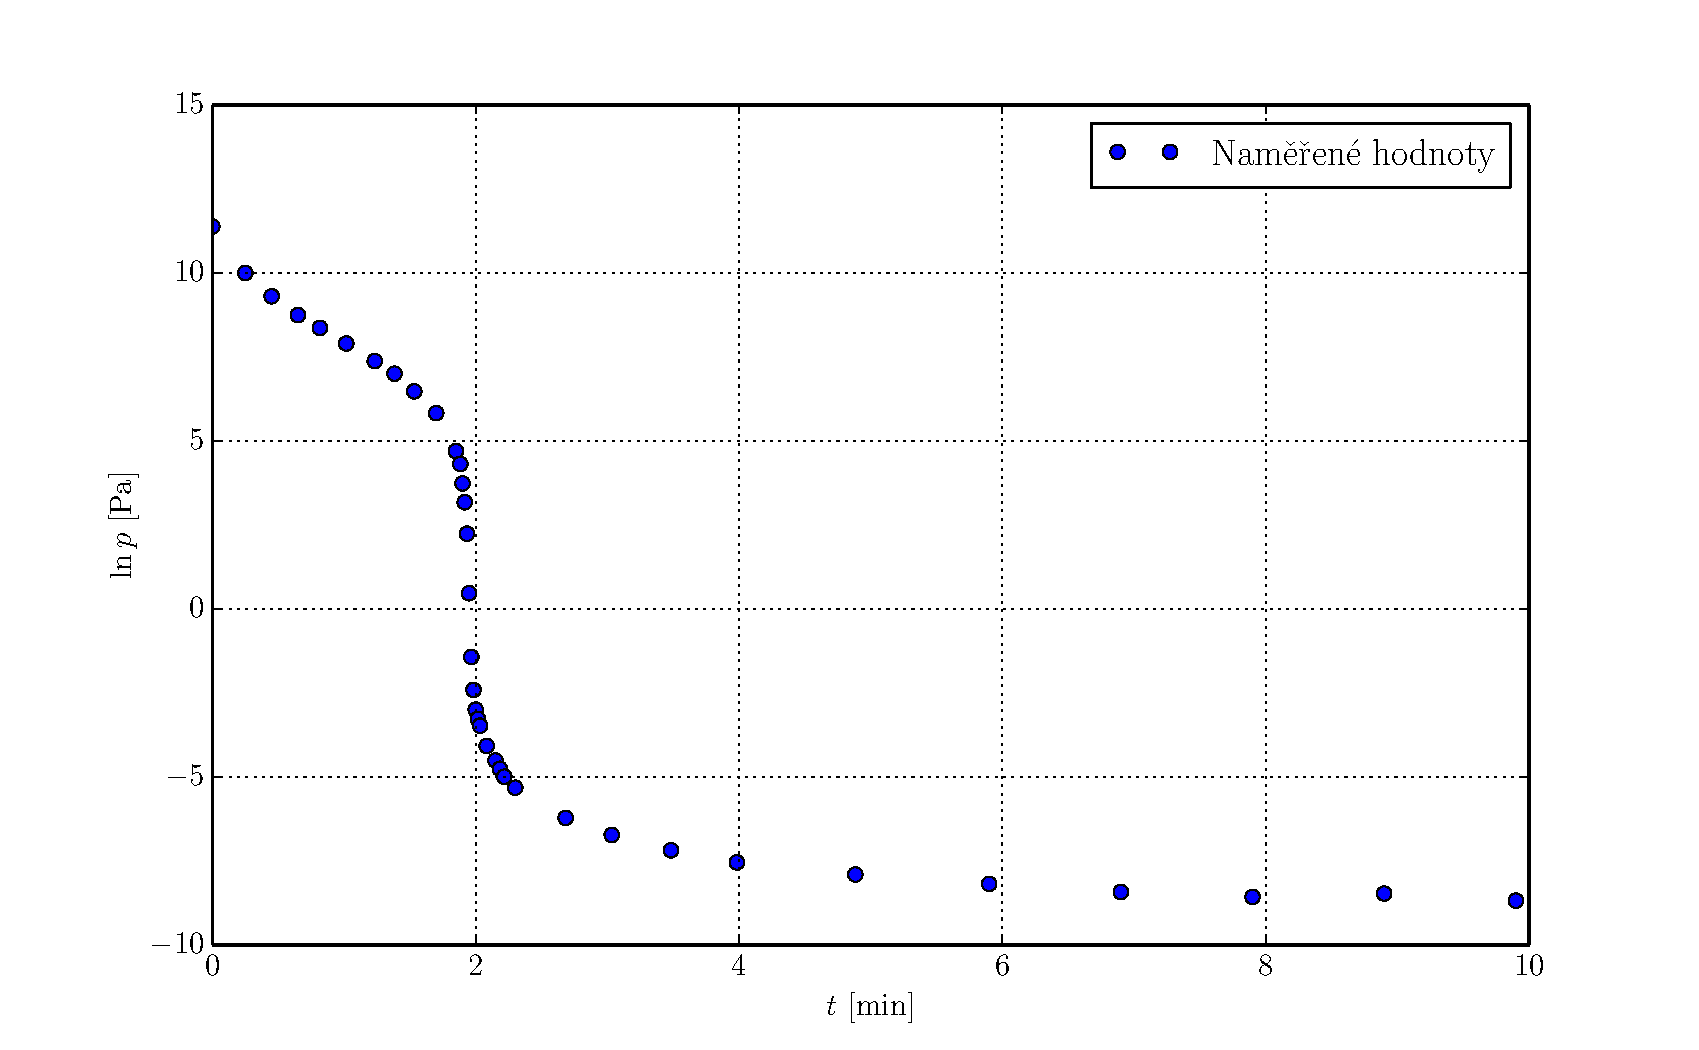
\includegraphics[width=\linewidth]{../plt/04_lnp.pdf}
		\vspace*{-0,7cm}
		\caption{Graf závislosti $\ln p$ na čase při čerpání TMV; $p$ je tlak zaznamenávaný v recipientu. }
		\label{fig:g_lnp}
	\end{center}
\end{figure}

\begin{figure}[h!]
	\begin{center}
		\vspace*{-1cm}
		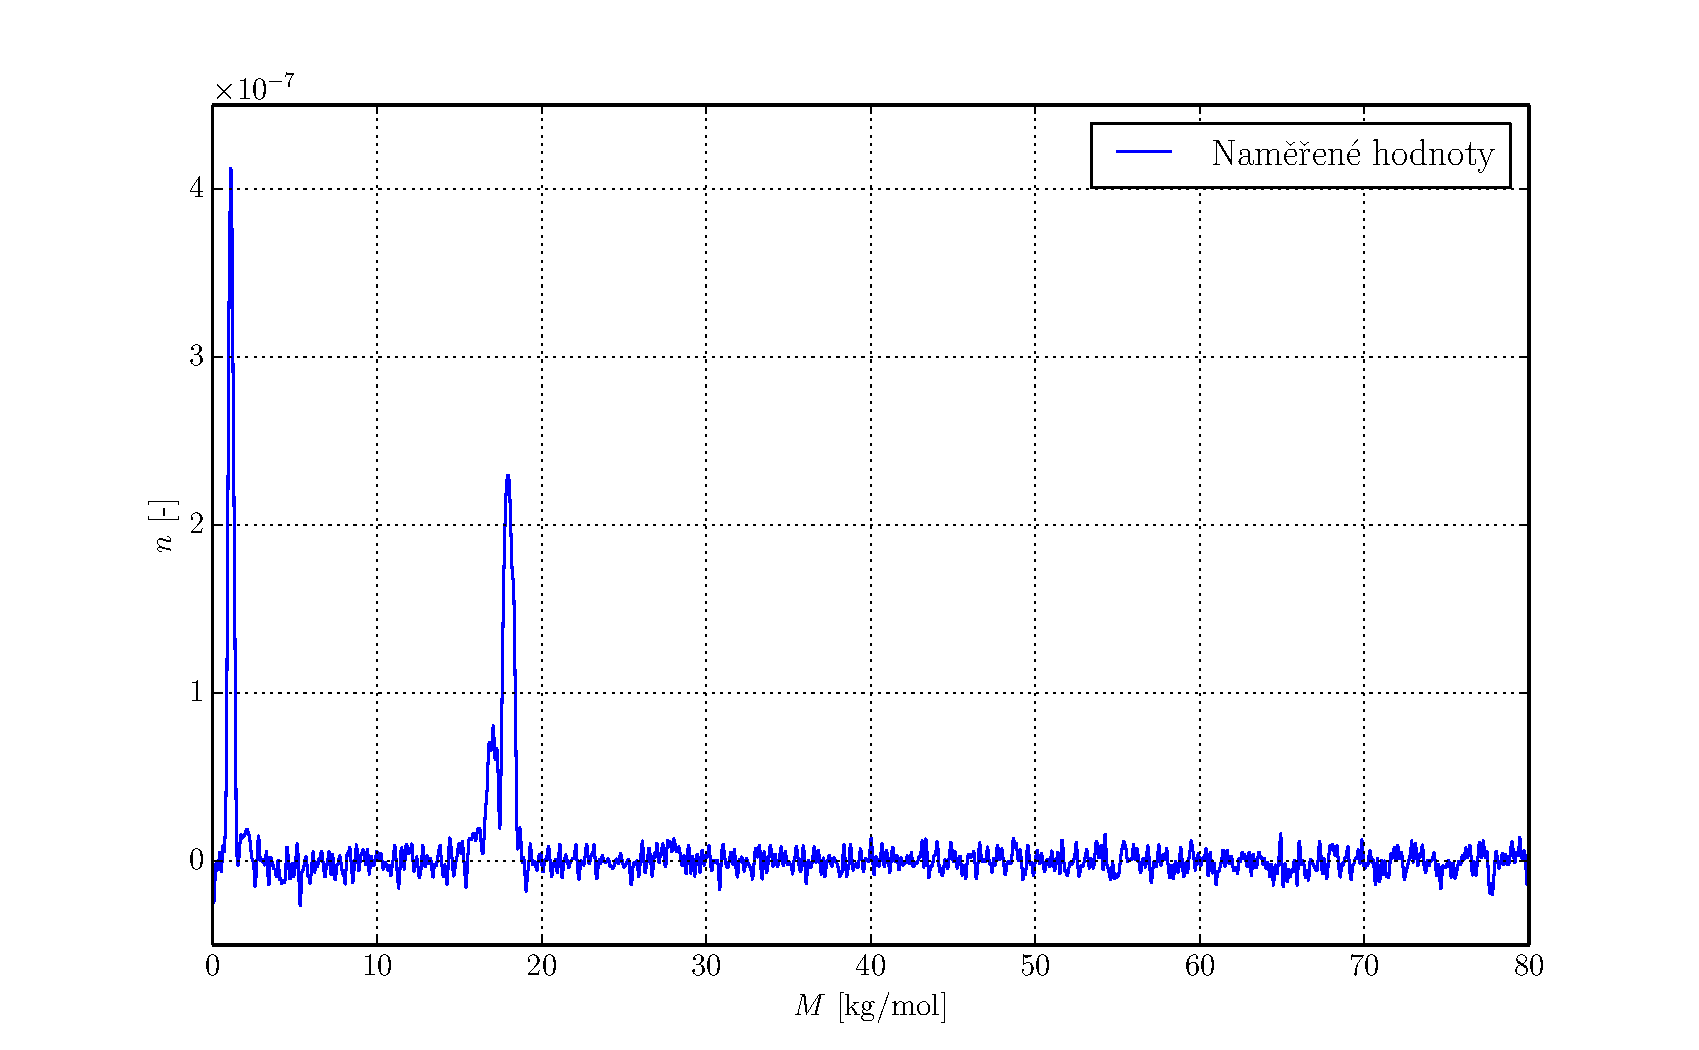
\includegraphics[width=\linewidth]{../plt/01_test.pdf}
		\vspace*{-0,7cm}
		\caption{Graf hmotnostního spektra zbytkového plynu; $n$ je četnost plynu, $M$ jeho molární hmotnost. } %Záznam jsme pořídili pomocí programu $\mathrm{Talk Star}$. }
		\label{fig:g_spektrum}
	\end{center}
\end{figure}


\begin{figure}[h!]
	\begin{center}
		\vspace*{-1cm}
		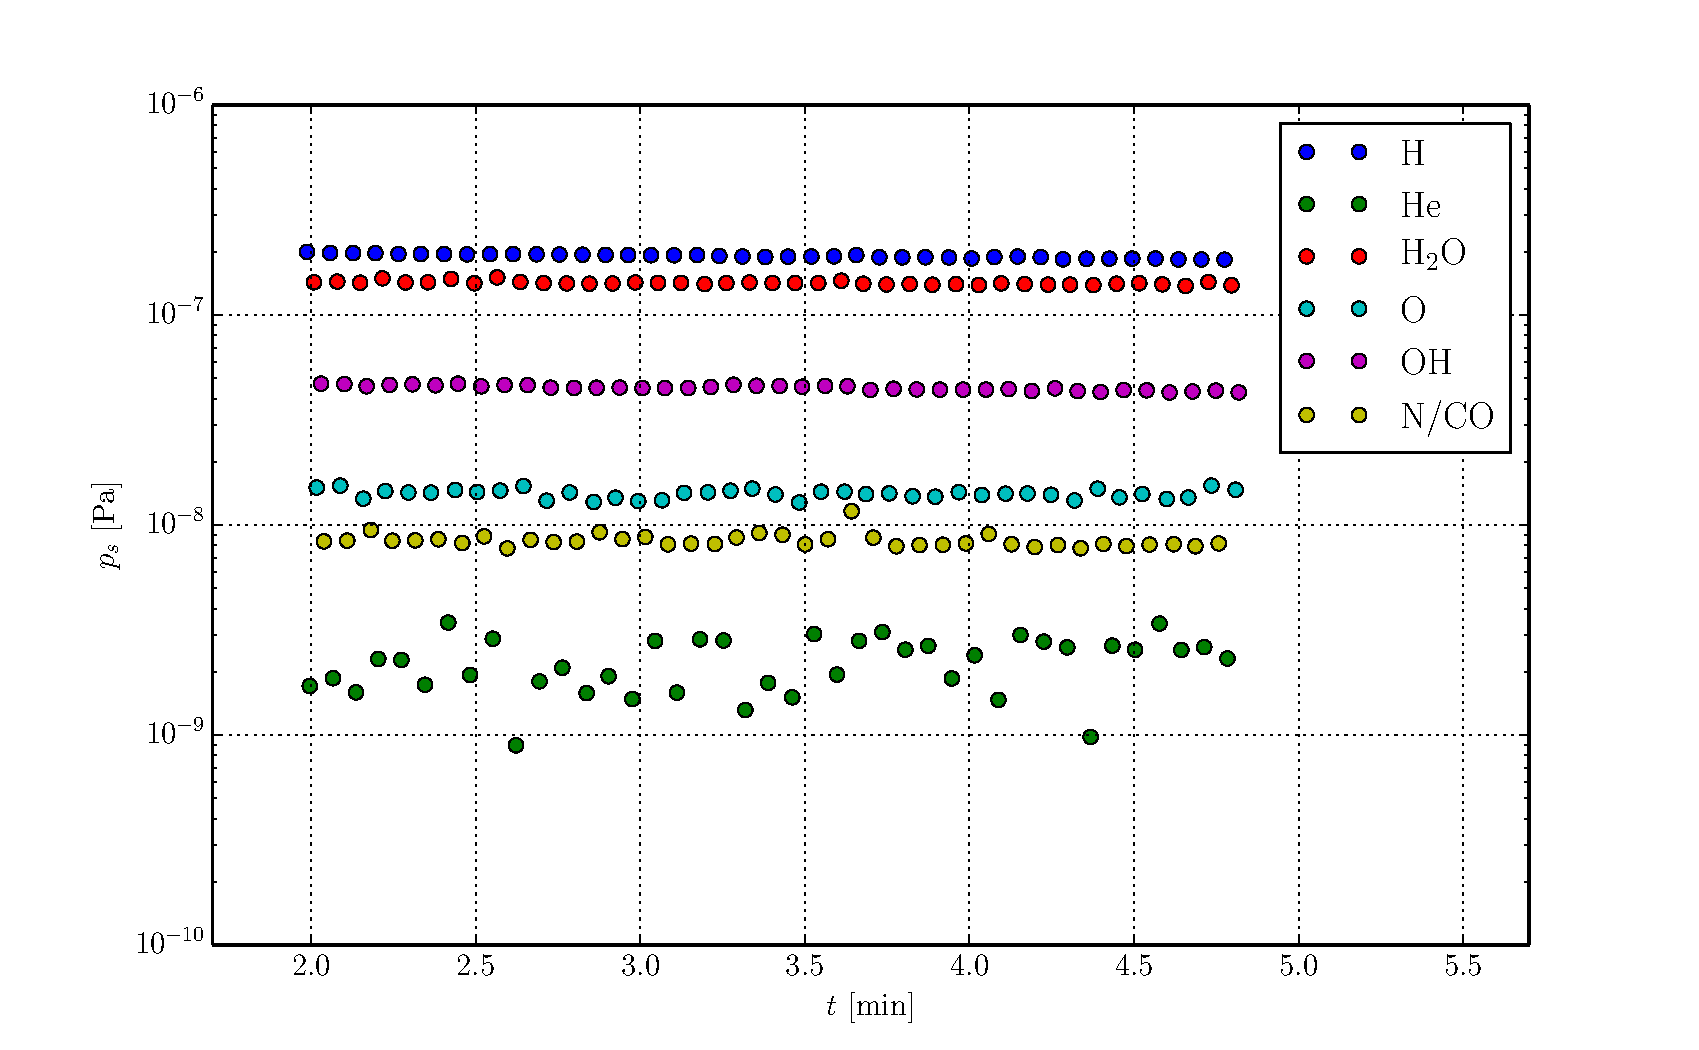
\includegraphics[width=\linewidth]{../plt/05_trend.pdf}
		\vspace*{-0,8cm}
		\caption{Graf závislosti parciálních tlaků $p_s$ na čase $t$ při sledování recipientu v módu ,,Trend~2``. Ke všem hodnotám byla přičtena absolutní hodnota dvojnásobku nejnižší naměřené hodnoty pro $\mathrm{He}$.}
		\label{fig:g_trend}
	\end{center}
\end{figure}

\begin{figure}[h!]
	\begin{center}
		\vspace*{-1.5cm}
		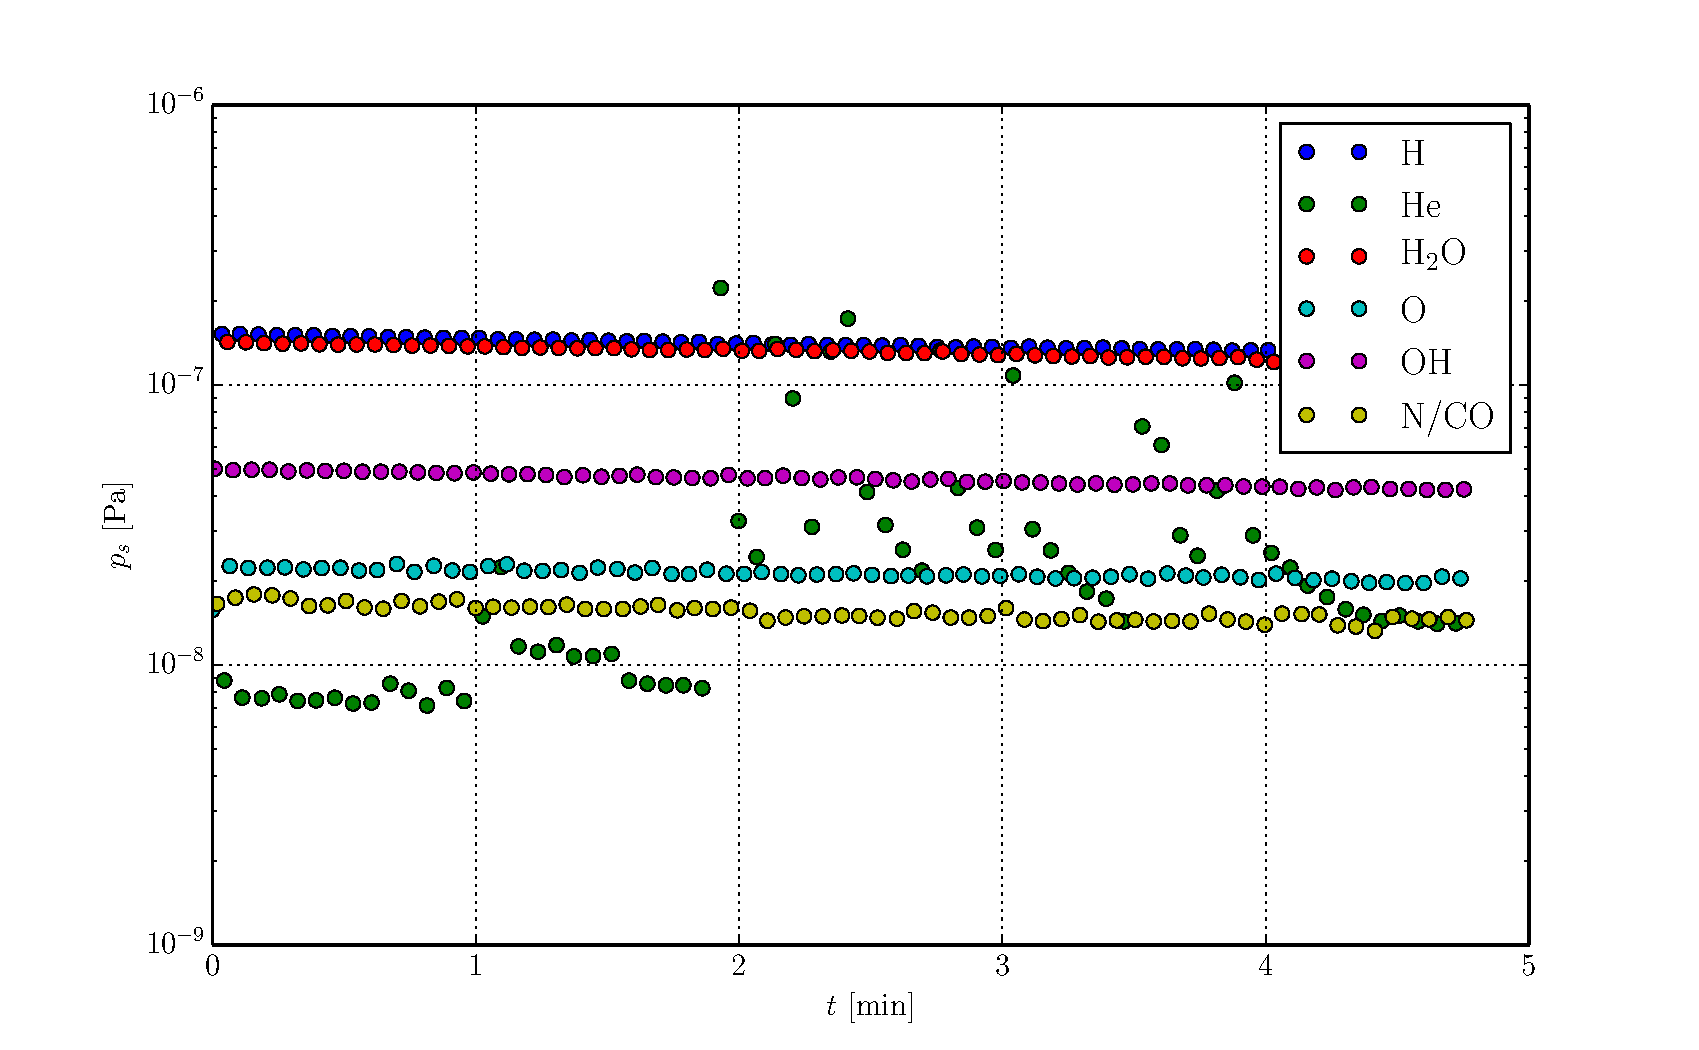
\includegraphics[width=\linewidth]{../plt/06_foukani.pdf}
		\vspace*{-0.8cm}
		\caption{Graf závislosti parciálních tlaků $p_s$ na čase $t$ při ofukování pootevřeného ventilu heliem. Ke všem hodnotám byla přičtena absolutní hodnota dvojnásobku nejnižší naměřené hodnoty pro $\mathrm{He}$. } %Záznam jsme pořídili pomocí programu $\mathrm{Talk Star}$. }
		\label{fig:g_foukani}
	\end{center}
\end{figure}

\begin{figure}[h!]
	\begin{center}
		\vspace*{-1.5cm}
		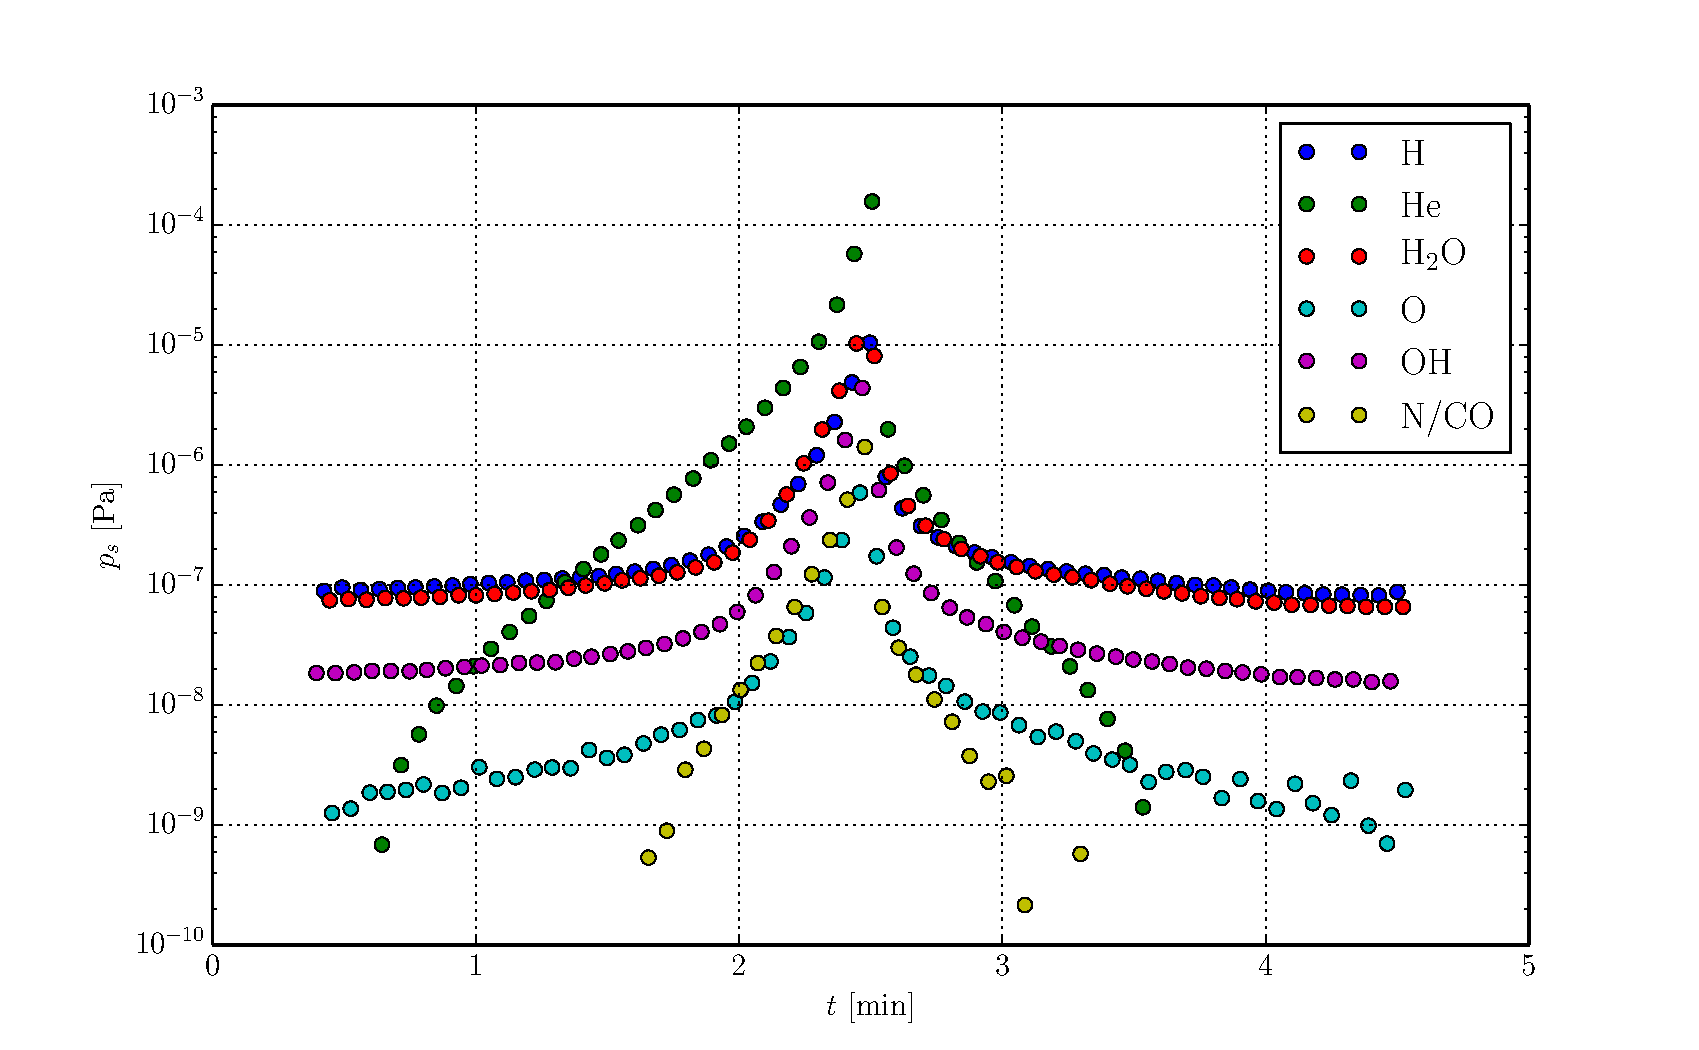
\includegraphics[width=\linewidth]{../plt/03_otacky.pdf}
		\vspace*{-0.8cm}
		\caption{Graf závislosti parciálních tlaků $p_s$ na čase $t$ při sledování vlivu změny otáček na složení zbytkové atmosféry. } %Záznam jsme pořídili pomocí programu $\mathrm{Talk Star}$. }
		\label{fig:g_otacky}
	\end{center}
\end{figure}

\begin{figure}[h!]
	\begin{center}
		\vspace*{-1.5cm}
		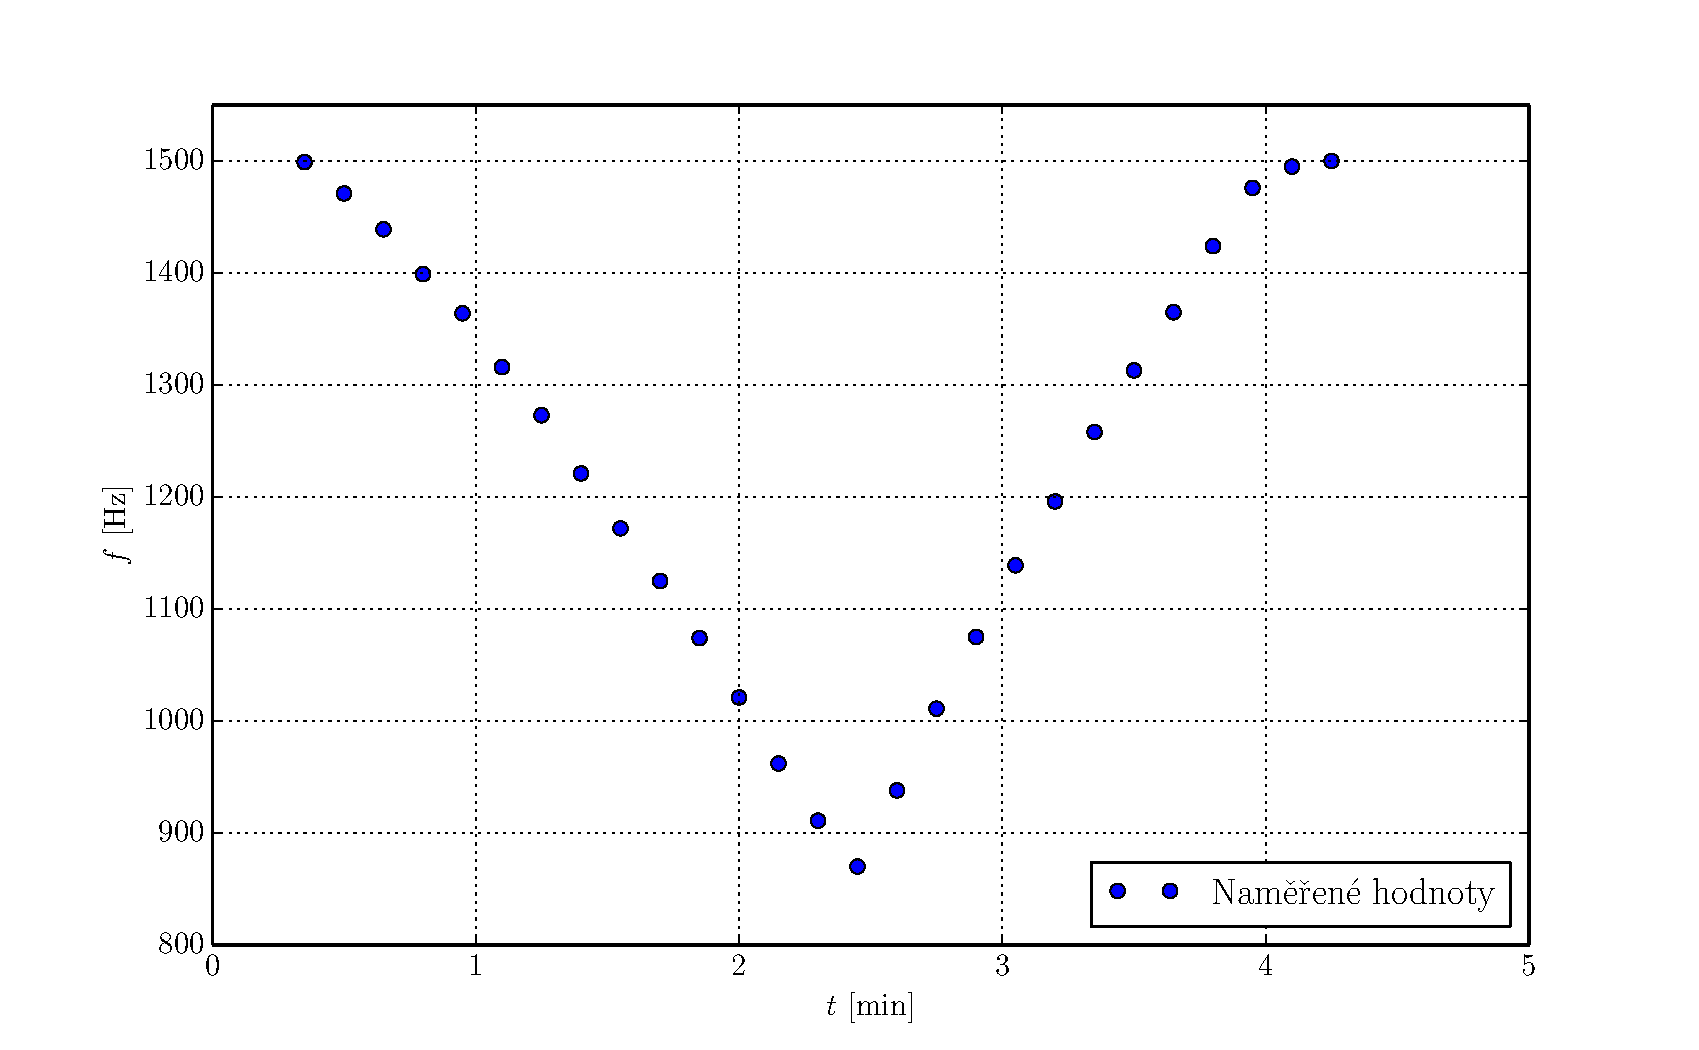
\includegraphics[width=\linewidth]{../plt/03_otacky_1.pdf}
		\vspace*{-0.8cm}
		\caption{Graf závislosti frekvence TMV $f$ na čase $t$ při sledování vlivu změny otáček na složení zbytkové atmosféry. } %Záznam jsme pořídili pomocí programu $\mathrm{Talk Star}$. }
		\label{fig:g_otacky_1}
	\end{center}
\end{figure}

% --- Konec dokumentu --------------------------------------------------

\end{document}

